No existe una definición universalmente aceptada de lo que configura discurso de odio. Para intentar acercarnos lo más posible a este concepto, en esta sección haremos un repaso muy general de algunos tratados internacionales sobre la materia, a la vez que también haremos un racconto de las definiciones utilizadas en trabajos dedicados a abordar este problema mediante herramientas de procesamiento de lenguaje natural.

\tbf{Una pequeña aclaración:} en la normativa sobre derechos humanos muchas veces se encuentra delimitado el discurso \tbf{discriminatorio} del discurso de \tbf{odio}, siendo este último una subcategoría del primero de mayor intensidad y con incitaciones a la violencia contra grupos protegidos o individuos miembros de estos grupos. En la literatura de NLP sobre el tema se utiliza la expresión discurso de odio (\emph{hate speech}) para referirse indistintamente a ambos fenómenos.

Aún cuando entendemos que la acepción general del discurso de odio es puede entenderse como incorrecta desde la perspectiva de tratados internacionales, teniendo en cuenta que esta tesis está centrada en técnicas para su detección automática usaremos esta terminología para plegarnos a los usos y costumbres de la comunidad de NLP.

\subsection{Abordaje desde una perspectiva legal y de los Derechos Humanos}

Un principio general que hace a los derechos más elementales del hombre y a la vida en sociedad es la posibilidad de expresarse libremente, el \tbf{derecho a la libre expresión}. Este derecho está protegido por constituciones nacionales y numerosos tratados internacionales. Uno de estos tratados, el Pacto Internacional de Derechos Civiles y Políticos (\emph{ICCPR} por sus siglas en inglés) \footnote{Este pacto desarrolla los derechos civiles y políticos establecidos por la Declaración Universal de los Derechos Humanos de la ONU}, sancionado en 1966 en la Asamblea de las Naciones Unidas y ratificado por 166 países, incluye en su artículo 19:

\begin{displayquote}[Artículo 19 de la ICCPR]
1. Nadie podrá ser molestado a causa de sus opiniones.

2. Toda persona tiene derecho a la libertad de expresión; este derecho comprende la libertad de buscar, recibir y difundir informaciones e ideas de toda índole, sin consideración de fronteras, ya sea oralmente, por escrito o en forma impresa o artística, o por cualquier otro procedimiento de su elección.

3. El ejercicio del derecho previsto en el párrafo 2 de este artículo entraña deberes y responsabilidades especiales. Por consiguiente, puede estar sujeto a ciertas restricciones, que deberán, sin embargo, estar expresamente fijadas por la ley y ser necesarias para:

a) Asegurar el respeto a los derechos o a la reputación de los demás;

b) La protección de la seguridad nacional, el orden público o la salud o la moral públicas.
\end{displayquote}

Este artículo que garantiza el derecho a la libertad de expresión da cuenta también de que esta libertad no es completamente irrestricta. El ejercicio de los derechos e igualdad ante la ley de otros marca este límite, no pudiéndose utilizar esta libertad de expresión para avasallar los derechos de terceros. La Convención Internacional sobre toda forma de Discriminación Racial (ICERD) \footnote{\url{http://servicios.infoleg.gob.ar/infolegInternet/anexos/120000-124999/122553/norma.htm}} dice en su artículo 4 al respecto:

\begin{displayquote}[Artículo 4, ICERD]

Los Estados partes condenan toda la propaganda y todas las organizaciones que se inspiren en ideas o teorías basadas en la superioridad de una raza o de un grupo de personas de un determinado color u origen étnico, o que pretendan justificar o promover el odio racial y la discriminación racial, cualquiera que sea su forma, y se comprometen a tomar medidas inmediatas y positivas destinadas a eliminar toda incitación a tal discriminación o actos de tal discriminación y, con ese fin, teniendo debidamente en cuenta los principios incorporados en la Declaración Universal de Derechos Humanos, así como los derechos expresamente enunciados en el artículo 5 de la presente Convención, tomarán, entre otras, las siguientes medidas:

a) Declararán como acto punible conforme a la ley, toda difusión de ideas basadas en la superioridad o en el odio racial, toda incitación a la discriminación racial así como todo acto de violencia o toda incitación a cometer tal efecto, contra cualquier raza o grupo de personas de otro color u origen étnico, y toda asistencia a las actividades racistas, incluida su financiación;

b) Declararán ilegales y prohibirán las organizaciones, así como las actividades organizadas de propaganda y toda otra actividad de propaganda, que promuevan la discriminación racial e inciten a ella y reconocerán que la participación en tales organizaciones o en tales actividades constituye un delito penado por la ley;

c) No permitirán que las autoridades ni las instituciones públicas nacionales o locales, promuevan la discriminación racial o inciten a ella.
\end{displayquote}


Los Estados y otros organismos deben tomar medidas para poder asegurar el libre ejercicio de los derechos y la igualdad de todos sus miembros, aún cuando esto pueda significar una restricción en la libertad de expresión \cite{article192015}. Entendiendo entonces que el derecho a la expresión tiene sus límites, podemos pensar que el discurso de odio es una de esas fronteras. Si bien el discurso de odio es algo que no está completamente delimitado, repasaremos algunas definiciones de este fenómeno hechas en tratados para acercarnos un poco más a las características comunes que comparten las diferentes definiciones. La Observación General 35 del Comité por la Eliminación de la Discriminación Racial de la ONU (CERD) considera que será discurso de odio, y debe ser tipificado penalmente:

\begin{displayquote}[Recomendación 35 del Comité por la Eliminación de la Discriminación Racial, CERD]

    a) Toda difusión de ideas basada en la superioridad o en el odio racial o étnico, por cualquier medio;

    b) La incitación al odio, el desprecio o la discriminación contra los miembros de un grupo por motivos de su raza, color, linaje, u origen nacional o étnico;

    c) Las amenazas o la incitación a la violencia contra personas o grupos por los motivos señalados en el apartado anterior;

    d) La expresión de insultos, burlas o calumnias contra personas o grupos, o la justificación del odio, el desprecio o la discriminación por los motivos señalados en el apartado b) anterior, cuando constituyan claramente incitación al odio o a la discriminación;

    e) La participación en organizaciones y actividades que promuevan e inciten a la discriminación racial.
\end{displayquote}

%\citet{gagliardone2015countering} presenta un análisis de diversos organismos y sus definiciones de discurso de odio.

En líneas generales, como se menciona en el reporte de la CIDH sobre discurso de odio contra lesbianas, gay, trans e intersex en Latinoamérica \cite{CIDH2015}, el concepto usualmente es referido a expresiones que incitan a tomar algún tipo de medida hostil contra una víctima o un grupo de personas, siendo esta perteneciente a un determinado grupo social definido por laguna característica. Dicho esto, podría delimitarse el discurso discriminatorio del discurso de odio por la componente de la promoción e instigación de la violencia; sin embargo, para los fines de este trabajo utilizaremos los términos indistintamente. Aún cuando el discurso no contenga arengas ni incitaciones a cometer actos violentos, puede entenderse ese discurso como generador de un ambiente hostil y de intolerancia que termine promoviendo estos ataques físicos \cite{CIDH2015}.

\citet{article192015} condensa muchas de estas definiciones de una manera succinta, desglosando esto en ``odio'' y ``discurso'':

\begin{displayquote}[Article 19: Hate Speech Toolkit]
    1. Odio: emoción intensa e irracional de oprobio, enemistad y aborrecimiento hacia una persona o grupo de personas, por tener determinadas características protegidas (reconocidas en el derecho internacional), reales o percibidas. El “odio” es más que un mero prejuicio y debe ser discriminatorio. El odio es una muestra de un estado emocional u opinión y, por lo tanto, se diferencia de cualquier acto o acción que se haya llevado a cabo.
    2. Discurso: cualquier expresión que vierta opiniones o ideas, que comparte una opinión o una idea interna con un público externo. Puede adoptar muchas formas: escrita, no-verbal, visual o artística y puede ser difundida en los medios, incluyendo Internet, material impreso, radio o televisión.
\end{displayquote}

%%
%%
%% Link
%% https://docs.google.com/drawings/d/149dpb2nrvmFgWZJYcrToAxO4M5n7JNQInfWd62kw3jc/edit
%%
%%

\begin{figure}[t]
    \centering
    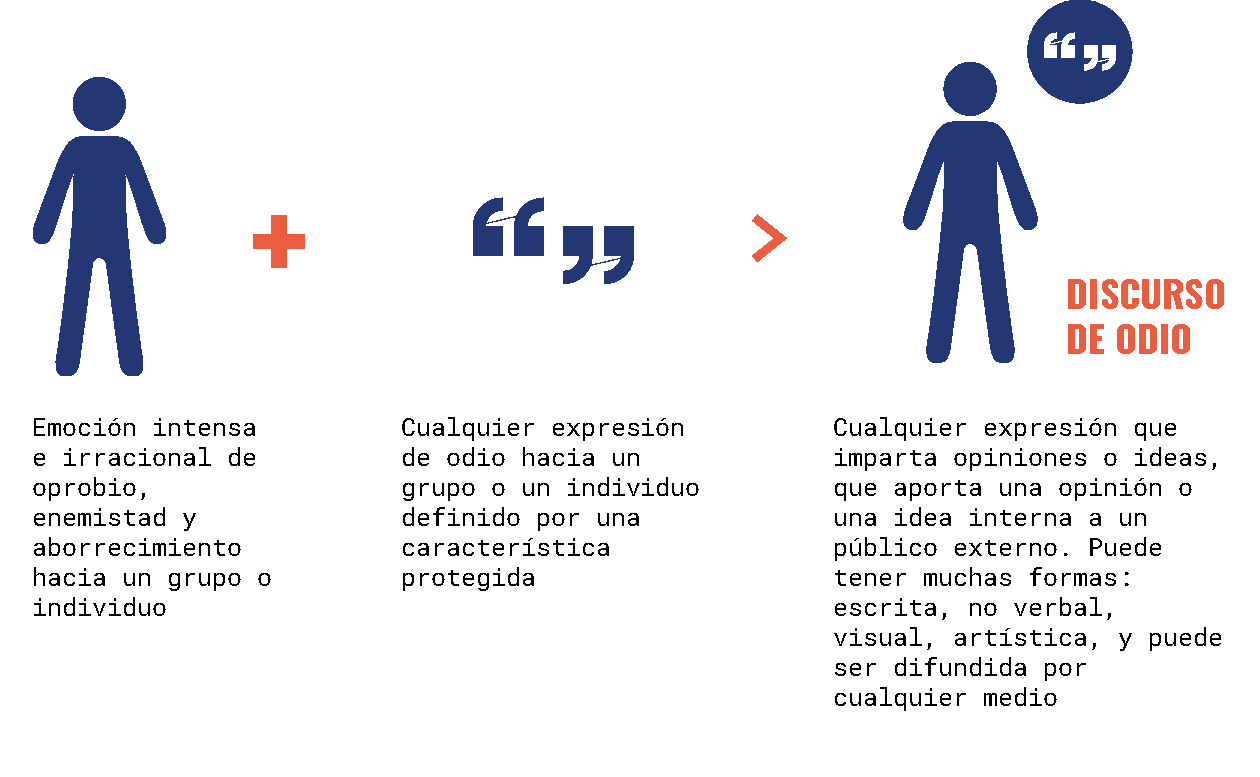
\includegraphics[width=\textwidth]{img/discurso_de_odio.pdf}
    \caption{Definición de discurso de odio de acuerdo al Toolkit de Article 19}
    \label{fig:hate_speech_definition_article_19}
\end{figure}


En base a esta definición, puede entenderse al discurso de odio como un discurso de cierta intensidad e irracionalidad que ataca a una persona o un grupo de personas por alguna característica históricamente vulnerada: por ser mujer, por su género, por su etnia, nacionalidad, religión, idioma, etc. La clave está en la combinación: un discurso irracional e intenso contra alguien que no posea una característica protegida no configura discurso de odio; por ejemplo, ataques a ciertas personas por ser periodistas. La figura \ref{fig:hate_speech_definition_article_19} ilustra esta definición.

No todo ataque a un individuo o una persona de algún colectivo discriminado es discurso de odio. En particular, la CIDH \cite{CIDH2015} menciona en base al informe de la UNESCO sobre discurso de odio \cite{gagliardone2015countering} que:

\begin{displayquote}[]
    (...) el discurso de odio no puede abarcar ideas amplias y abstractas, tales como las visiones e ideologías políticas, la fe o las creencias personales. Tampoco se refiere simplemente a un insulto, expresión injuriosa o provocadora respecto de una persona. Así definido, el discurso de odio puede ser manipulado fácilmente para abarcar expresiones que puedan ser consideradas ofensivas por otras personas, particularmente por quienes están en el poder, lo que conduce a la indebida aplicación de la ley para restringir las expresiones críticas y disidentes. Asimismo, el discurso de odio tiene que distinguirse de aquellos “crímenes de odio” que se basan en conductas expresivas, como las amenazas y la violencia sexual, y que se encuentran fuera de cualquier protección del derecho a la libertad de expresión
\end{displayquote}

Como vemos, no sólamente es difusa la frontera fijada la característica sobre qué es discurso de odio o insultos, sino que incluso también es difícil definir qué característica es protegida o no. En el siguiente capítulo hablaremos más de esto al describir los criterios utilizados a la hora de anotar un conjunto de datos sobre comentarios en Twitter.

\subsection{Definiciones utilizadas desde NLP}

